\documentclass[residuals.tex]{subfiles}

% Load any packages needed for this document
\begin{document}
	\large
\section*{Simple Linear Regression - Revision of Previous Material}	
In simple linear regression, we predict values on one variable from the values of a second variable. 

\begin{itemize}
	\item The variable we are predicting is called the \textbf{\textit{dependent variable}} (or response variable) and is referred to as Y. 
	
	\item The variable we are basing our predictions on is called the \textbf{i\textit{ndependent variable}} (or predictor variable) and is referred to as X.
\end{itemize} \textit{
\noindent Remark: When there is only one predictor variable, the prediction method is called simple regression. Linear regression can have more than one predictor variable, i.e. Multiple Linear Regression.}

\bigskip 
\noindent In simple linear regression, the predicted values of Y when plotted as a function of X form a straight line on the scatter plot. This line is known as the \textbf{\textit{regression line}}. 

\begin{figure}[h!]
	\centering
	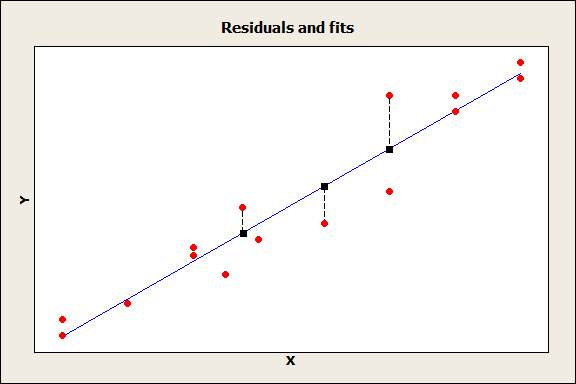
\includegraphics[width=0.9\linewidth]{resids1}
	\caption{}
	\label{fig:resids1}
\end{figure}

\begin{itemize}
	\item Suppose we construct our model using $n$ observed values of the response variable $y_1, y_2, \ldots y_i \ldots y_n$
	
	\item For the original data set, there is a predicted value of each case of $Y$ that corresponds to an observed value of $Y$. 
	
	\item The difference between an observed value of the dependent variable ($y_i$) and the corresponding predicted value ($\hat{y}$) is called the residual ($e_i$). Each data point from the data set has one residual.
	
	\item Simply put, the values of the residuals are derived as follows: 
	\[\mbox{Residual = Observed value - Predicted value}\]
	\[e_i = y_i - \hat{y_i} \]
	\item For three cases in the graphic above, the observed value (red dot) is linked to its corresponding predicted value (black dot) on the regression line (blue line).
	The difference (i.e. residual) is depicted using a dashed line. The magnitude of these residuals is of interest.
	\item The second of the three residuals will have a negative value.
	\item \textbf{\textit{Ordinary Least Squares}} is a method of fitting a model, such that the total residual values are minimised.
	
	
	\item Important theoretical assumption underlying the OLS model: the sum of the residuals should equal to zero. 
	
	{
		\Large
		\[\sum e_i = 0\]
	}
	\item An extension of this is that the expected value of the residuals is 0. 
	$\mathrm{E}(e) = 0$
	\item Another Important Theoretical Assumption - The residuals are normally distributed. (more on that later)
\end{itemize}
\newpage
\section*{Statistical Assumptions for Linear Models}
%\subsection{Statistical Assumptions}
The assumptions of multiple linear regression analysis are similar to those of the simple case involving only one independent variable. For point estimation, the principal assumptions are that


\begin{itemize}
	\item[(1)] the dependent variable is a continuous random variable ,
	\item[(2)] the relationship between the several independent variables and the one dependent variable is \textit{linear} (as opposed to quadratic or cubic - this is something we will explore more later).
\end{itemize}
\begin{figure}[h!]
\centering
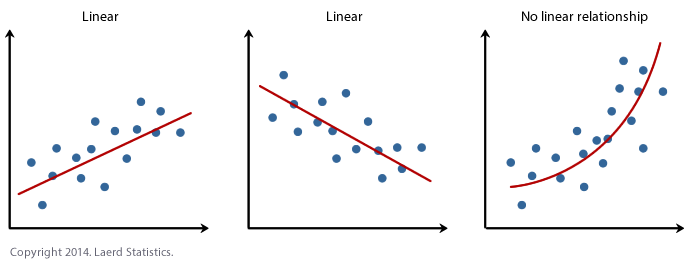
\includegraphics[width=0.7\linewidth]{linear-nonlinear-relationships}
\end{figure}

\noindent Additional assumptions for statistical inference (estimation or hypothesis testing) are that
\begin{itemize}
	\item[(3)] the variances of the conditional distributions of the dependent variable, given various combinations of values of the independent variables, are all equal,
	\item[(4)] the conditional distributions of the dependent variable
	are normally distributed (\textit{i.e. Residuals are nomally distributed}),
	\item[(5)] the observed values of the dependent variable are independent of each other. (\textit{Violation of this assumption is called autocorrelation.} 
\end{itemize}
\newpage
\section*{Polynomial Regression}
Polynomial regression is an extension of linear regression in which the relationship between the independent variable $X$ and the dependent variable $Y$ is modelled as an $n-$th degree polynomial (e.g. a quadratic or cubic function).  You may tryout out various types of polynomial regression if a linear relationship proves unsatisfactory.

\begin{itemize}
\item Simple Linear regression (degree n=1)
\[
\hat{y} = b_0 + b_1 x \]
\item quadratic relationship (degree n=2)
\[
\hat{y} = b_0 + b_1 x + b_2 x^2 \]
\item cubic relationship (degree n=3)
\[
\hat{y} = b_0 + b_1 x + b_2 x^2 + b_1 x^3 \]
\end{itemize}

To determine which model suits the data the best, you can try model metrics such as the AIC and adjusted R-squared.


\newpage
%--------------------------------------------------------------------------------------%
\section*{Model Validation}
%http://www.itl.nist.gov/div898/handbook/pmd/section4/pmd44.htm
\begin{itemize}
\item Model validation is possibly the most important step in the model building sequence. It is also one of the most overlooked. Often the validation of a model seems to consist of nothing more than quoting the $R^2$ statistic from the fit (which measures the fraction of the total variability in the response that is accounted for by the model). 

\item Unfortunately, a high $R^2$ value does not guarantee that the model fits the data well. Use of a model that does not fit the data well cannot provide good answers to the underlying engineering or scientific questions under investigation.

\item Model diagnostic techniques determine whether or not the distributional assumptions are satisfied, and to assess the influence of unusual observations.

\end{itemize}


\subsection*{Why Use Residuals?}

If the model fit to the data were correct, the residuals would approximate the random errors that make the relationship between the explanatory variables and the response variable a statistical relationship. Therefore, if the residuals appear to behave randomly, it suggests that the model fits the data well. On the other hand, if non-random structure is evident in the residuals, it is a clear sign that the model fits the data poorly. 

%The subsections listed below detail the types of plots to use to test different aspects of a model and give guidance on the correct interpretations of different results that could be observed for each type of plot.
%%------------------------------------------------------------------------------------------------------------------------ %
\section{Introduction to Residuals}

The difference between the observed value of the dependent variable (y) and the predicted value ($\hat{y}$) is called the \textbf{residual} (e). Each data point has one residual.

\begin{framed}
\[\mbox{Residual} = \mbox{Observed value} - \mbox{Predicted value}\] 
\[e = y - \hat{y}\]
\end{framed}

Both the sum and the mean of the residuals are equal to zero. 
%That is, Σ e = 0 and e = 0.
\newpage

\subsection*{Residual Plots}
\begin{itemize}
\item A residual plot is a graph that shows the residuals on the vertical axis and the independent variable on the horizontal axis. \item If the points in a residual plot are randomly dispersed around the horizontal axis, a linear regression model is appropriate for the data; otherwise, a non-linear model is more appropriate.

\item Below the table on the left shows inputs and outputs from a simple linear regression analysis, and the chart on the right displays the residual (e) and independent variable (X) as a residual plot.
\end{itemize}

\begin{center}
\begin{tabular}{|c|c|c|c|c|c|}
	\hline   x	& 60	& 70	& 80	& 85 &	95 \\ \hline
	y	& 70	& 65	& 70	& 95 &	85 \\ \hline
	$\hat{y}$	& 65.411 & 	71.849	& 78.288	& 81.507	& 87.945 \\ \hline
	e	& 4.589	& -6.849 &	-8.288&	13.493	& -2.945 \\ \hline
\end{tabular} 
\end{center}
\begin{figure}[h!]
\centering
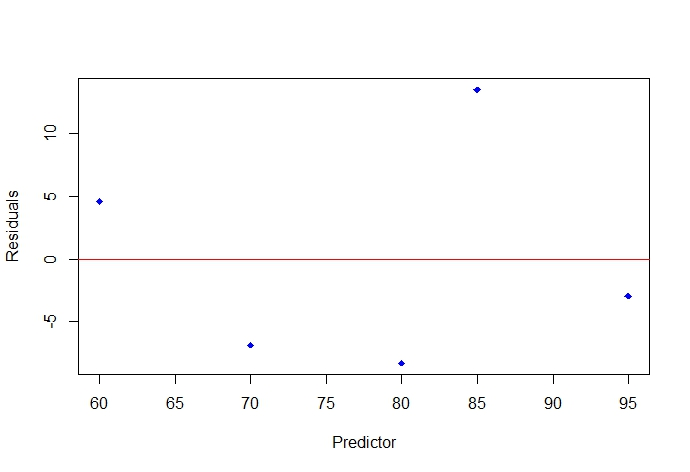
\includegraphics[width=0.7\linewidth]{residplotnew}

\end{figure}


The residual plot shows a fairly random pattern - the first residual is positive, the next two are negative, the fourth is positive, and the last residual is negative. This random pattern indicates that a linear model provides a decent fit to the data.

%============================================================================%
\newpage
\begin{itemize}
\item Below, the residual plots show three typical patterns. 
\item The first plot shows a random pattern, indicating a good fit for a linear model. 
\item The other plot patterns are non-random (U-shaped and inverted U), suggesting a better fit for a non-linear model.
\end{itemize}



		
\begin{figure}
\centering
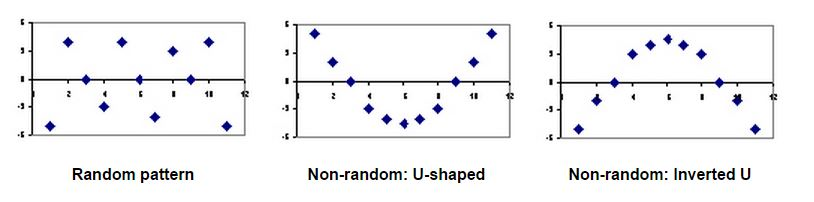
\includegraphics[width=0.7\linewidth]{residsplot-typs}
\end{figure}




\end{document}